\documentclass[12pt, man]{apa6}
\usepackage[american]{babel}
\usepackage{csquotes}
\usepackage[style=apa,sortcites=true,sorting=nyt,backend=biber]{biblatex}
\usepackage{graphicx}
\DeclareLanguageMapping{american}{american-apa}
\addbibresource{ref.bib}


\abstract{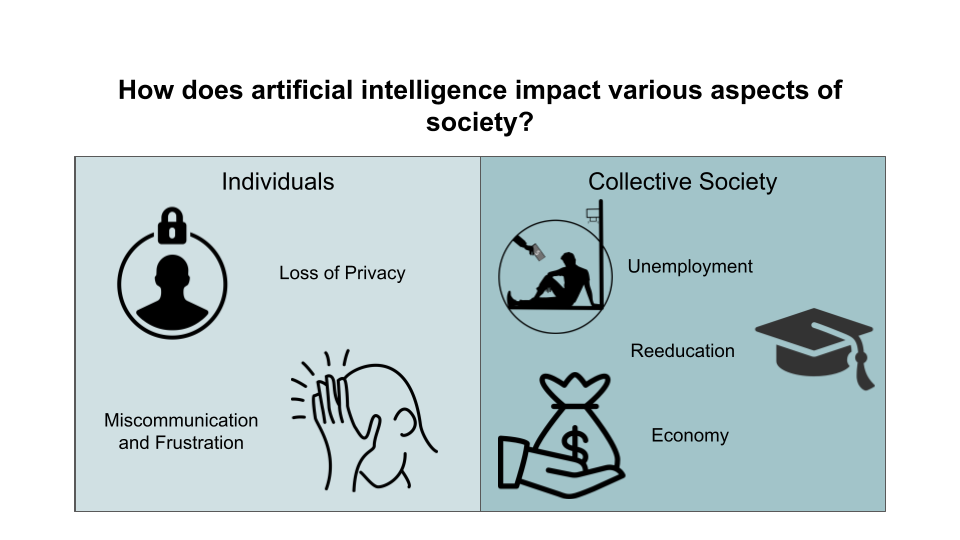
\includegraphics[width=\textwidth]{visualAbstract.png}}

\keywords{Artificial intelligence, automation, algorithms, data collection, economy, consumer, engagement, unemployment}

\title{The Impact of Artificial Intelligence on Society}
\shorttitle{AI and Society}

\author{Garrett Price}
\affiliation{Brigham Young University}

\rightheader{AI and Society}
\begin{document}
\maketitle

Artificial Intelligence has been misunderstood by the masses ever since the term was conceived.  Media has greatly exaggerated the potential
benefits and drawbacks to this AI revolution.  These misconceptions of what artificial intelligence is and can do lead to concern. Many people question
whether AI has a place in our world and do not fully understand the benefits. Others are eager to implement automation in many aspects but are unaware of the
potential drawbacks.  For the purposes of this article, artificial intelligence refers to any form of automation by technology, such as cleaning robots or algorithms used on social media sites to display certain posts.\\
How has AI truly affected society and what needs to be done about it? This article seeks to address this question by combining the findings of studies from across the globe to clarify how AI can impact various aspects of life.  While the available research is extensive, it cannot provide a definitive answer of how AI will impact society due to the rapidly evolving nature of the field.  However, the results and conclusions from the current studies do provide enough information to see how AI has affected society up until now.  These effects can be changed according to how governments, tech firms, and employees react to the growing influence of AI.  This paper will address how AI has affected many aspects of life including consumer interactions, employment opportunities, and national economies.  It will discuss who benefits from automation and who is harmed by automation in each field.  The potential actions that can be taken to maximize or minimize the impact in each area will also be discussed.  First, the impact on individuals will be analyzed.  How AI can affect individuals in their consumer experiences.  Next, the effects of artificial intelligence on society as a whole will be addressed.  These effects include economic changes and the spread of misinformation.  Lastly, the possible actions that governments, businesses, and individuals can make to limit or expand the effects of AI in the stated fields.
\newpage
\section*{Impact of AI on Individuals}
Consumers are having more interactions with AI as businesses automate more aspects of the consumer experience.  Any situation in which a consumer interacts with an AI, knowingly or not, to achieve something can be considered when discussing AI's impact on consumers.\\
\subsection*{Personalized Experiences and Loss of Privacy}
The use of AI to collect and analyze data in consumer experiences leads to very different interactions with each consumer \parencite{Puntoni2021}.  These personalized experiences can make it easier for consumers to get what they want.  For example, one heavily personalized experience would be a social media feed.  The implemented algorithms collect data of the user and are able to find similar posts that the user is more likely to interact with.
This type of interaction with AI can be good for the consumer if it is what they expect.  Receiving recommendations based on interests can lead to a more fulfilling experience for the consumer.  It can also forge a relationship between the consumer and the company \parencite{Kumar2019}.  However, this application of AI can lead to users feeling vulnerable and exploited if not handled properly.  Aguirre et al. \parencite*{Aguirre2015} made the observation that "covert data collection", or the act of collecting data without the consumer's knowledge or consent, causes users to feel uncomfortable and can backfire on the company as the consumer stops interacting with them due to loss of trust.

Puntoni et al. \parencite*{Puntoni2021} claimed that as technology has become more central to life, consumers lose more ownership of their own personal data. This collection of data causes people to fear a "surveillance state" where everything they do and say is being recorded.  This state has slowly become a reality as now words heard by speakers in the home to movies selected on Netflix are all fed to one company's AI or another to control what the user experiences next. As stated above, consumers are made very uncomfortable by covert data collection.  It starts to become a trade-off for people as they weigh the benefits of a tailor-made experience and the cost of losing ownership of personal data.

What needs to be done to make these experiences better for the individual?  Studies have shown that personalization leads to more interaction by consumers companies are more transparent with how they collect the user's data while no change was noted when companies use more covert strategies \parencite{Aguirre2015}.  For consumers to have a better experience with AI personalization companies must be up front with what data they are collecting and how it will be used.  There is currently no widely accepted standard of ethical use of AI in fields such as marketing\parencite{Puntoni2021}.  In order to protect consumers' privacy and personal data, there must be some sort of guideline for companies to follow on what is ethical or not.

\subsection*{Service AI and Consumers}
People want an AI to make certain tasks easier \parencite{Trivedi201991}.  For this section, chatbots, or AI that chat with users for purposes such as customer service, will be discussed.  They are a prime example of a service AI that attempts to make something easier for an individual and there has been much research on their effectiveness.  While only one example will be dissected, the same ideas to improve chatbot functionality can also be applied to other service AI.

Chatbots have many clear benefits for the consumer and for the business.  They allow for access to customer service at any hour, they are fast and efficient, and they are able to help more people than a human chat agent \parencite{McLean2017494}. These aspects make receiving customer support quick and easy for the consumer.  Trivedi \parencite*{Trivedi201991} observed that effective use of chatbots can also increase the trust consumers have in the company.  However, the "service quality, information quality, and system quality" customers experience impacts their interactions more than any of the benefits above \parencite{McLean2017494}.  No customer will leave feeling satisfied with the service they received from the AI if the information given was incorrect, the responses were slow, or the interface was difficult to understand.  The ideas of service, information, and system quality are important for determining how to improve the customer's experience with the service AI.  These aspects are able to be observed easily through surveys directed to the consumer or tests under various circumstances.  These should be the first things that companies seek to improve if they want a better experience for their customers.

Wirtz \parencite*{Wirtz2018} observed in a study that robots that can "mimic the expression" of the person that is interacting with them are perceived as more "pleasant" and customers are more willing to interact with them.  Mclean, Graeme, and Frimpong \parencite*{McLean2017494} observed a similar effect with their chatbot studies and the use of emoticons.  However, they do disagree about their importance.  Wirtz stated that the "warmth" of the service AI is as impactful as its ability.  Mclean claimed that 
\subsection*{Wages}
\subsection*{Reskilling and Upskilling}

\section*{Impact of AI on society}
\subsection*{Economic Impact}

\subsection*{Misinformation}

\printbibliography

\end{document}